\whiteBGstarBegin
\setcounter{section}{0}
\section{Lý thuyết: Quá trình đẳng áp}
\begin{enumerate}[label=\bfseries Câu \arabic*:]
	
	\item \mkstar{1} [5]
	
	\cauhoi{
		Hệ thức nào sau đây \textbf{không} phù hợp với quá trình đẳng áp?
		\begin{mcq}(4)
			\item $V\sim \dfrac{1}{T}$.
			\item $\dfrac{V}{T} = \text{hằng số}$.
			\item $\dfrac{V_1}{T_1} = \dfrac{V_2}{T_2}$.
			\item $V\sim T$.
		\end{mcq}
	}
	
	\loigiai{
		\textbf{Đáp án: A.}
		
		Hệ thức phù hợp với quá trình đẳng áp là $V\sim T$ hay $\dfrac{V}{T} = \text{hằng số}$ hay $\dfrac{V_1}{T_1}=\dfrac{V_2}{T_2}$.
	}

\item \mkstar{1} [5]

\cauhoi{
	Quá trình biến đổi trạng thái trong đó áp suất được giữ không đổi gọi là quá trình
	\begin{mcq}(4)
		\item đẳng tích.
		\item đẳng áp.
		\item đẳng nhiệt.
		\item đoạn nhiệt.
	\end{mcq}
}

\loigiai{
	\textbf{Đáp án: B.}
	
	Quá trình biến đổi trạng thái trong đó áp suất được giữ không đổi gọi là quá trình đẳng áp.
}
	\item \mkstar{1} [24]

\cauhoi{
	Trong quá trình đẳng áp, thông số trạng thái nào thay đổi?
	\begin{mcq}(2)
		\item Nhiệt độ và áp suất. 
		\item Nhiệt độ và thể tích.
		\item Thể tích và áp suất.
		\item Nhiệt độ, áp suất và thể tích.
	\end{mcq}
	
}

\loigiai{
	\textbf{Đáp án: B.}
	
	Trong quá trình đẳng áp, áp suất được giữ không đổi, nhiệt độ và thể tích thay đổi.
}
\item \mkstar{1} [24]

\cauhoi{
	Phương trình nào sau đây là phương trình trạng thái khí lí tưởng?
	\begin{mcq}(2)
		\item $\dfrac{VT}{p} = \text{hằng số}$. 
		\item $\dfrac{p_1V_2}{T_1} = \dfrac{p_2V_1}{T_2} = \text{hằng số}$.
		\item $\dfrac{pT}{V} = \text{hằng số}$.
		\item $\dfrac{pV}{T} = \text{hằng số}$.
	\end{mcq}
}

\loigiai{
	\textbf{Đáp án: D.}
	
	Phương trình trạng thái khí lí tưởng: $\dfrac{pV}{T} = \text{hằng số}$ hoặc $\dfrac{p_1V_1}{T_1} = \dfrac{p_2V_2}{T_2}$.
}

\item \mkstar{2} [5]

\cauhoi{
	Một khối khí có áp suất không đổi ở nhiệt độ $\SI{50}{\celsius}$. Nhiệt độ khối khí phải tăng đến bao nhiêu để thể tích tăng gấp đôi?
	\begin{mcq}(4)
		\item $\SI{200}{\celsius}$.
		\item $\SI{100}{\celsius}$.
		\item $\SI{373}{\celsius}$.
		\item $\SI{646}{\celsius}$.
	\end{mcq}
}

\loigiai{
	\textbf{Đáp án: ABC.}
	
	Đẳng áp (1): $V_1$, $T_1=\SI{323}{K}$ sang (2): $V_2=2V_1$, $T_2=?$
	
	Vì quá trình là đẳng áp nên ta có phương trình:
	
	$$\dfrac{V_1}{T_1} = \dfrac{V_2}{T_2} \Rightarrow T_2 =\dfrac{V_2T_1}{V_1} = \SI{646}{K}.$$
	
	Đổi $t_2=T_2-273 = \SI{373}{\celsius}$.
}

\item \mkstar{2} [5]

\cauhoi{
	Giữ áp suất của một khối lượng khí không thay đổi, để thể tích tăng lên gấp 3 lần thì nhiệt độ tuyệt đối
	\begin{mcq}(2)
		\item tăng lên 3 lần.
		\item giảm đi 3 lần.
		\item tăng lên 6 lần.
		\item giảm đi 6 lần.
	\end{mcq}
}

\loigiai{
	\textbf{Đáp án: A.}
	
	Đẳng áp (1): $V_1$, $T_1$ sang (2): $V_2=3V_1$, $T_2=?$
	
	Vì quá trình là đẳng áp nên ta có phương trình:
	
	$$\dfrac{V_1}{T_1} = \dfrac{V_2}{T_2} \Rightarrow T_2 =\dfrac{V_2T_1}{V_1} = 3T_1.$$
	
	Cách khác: Thể tích tỉ lệ thuận với nhiệt độ tuyệt đối, để thể tích tăng lên gấp 3 lần thì nhiệt độ tuyệt đối tăng gấp 3 lần.
}

\item \mkstar{2} [5]

\cauhoi{
	Một khối khí ở nhiệt độ $\SI{0}{\celsius}$, thể tích 5 lít. Khi nhiệt độ tăng thêm $\SI{60}{\celsius}$ thì thể tích của khối khí là bao nhiêu? Biết áp suất giữ không đổi.
	\begin{mcq}(4)
		\item $\SI{6.1}{l}$.
		\item $\SI{5.4}{l}$.
		\item $\SI{5.7}{l}$.
		\item $\SI{6.3}{l}$.
	\end{mcq}
}

\loigiai{
	\textbf{Đáp án: A.}
	
	Đẳng áp (1): $V_1=\SI{5}{l}$, $T_1=\SI{273}{K}$ sang (2): $V_2=?$, $T_2=\SI{333}{K}$
	
	Vì quá trình là đẳng áp nên ta có phương trình:
	
	$$\dfrac{V_1}{T_1} = \dfrac{V_2}{T_2} \Rightarrow V_2 =\dfrac{V_1T_2}{T_1} = \SI{6.1}{l}.$$
}

\item \mkstar{2} [5]

\cauhoi{
	Ở nhiệt độ $\SI{273}{\celsius}$ thể tích của một khối khí là 5 lít. Khi áp suất không đổi, thể tích của khối khí đó ở $\SI{546}{\celsius}$ là
	\begin{mcq}(4)
		\item $\SI{15}{l}$.
		\item $\SI{2.5}{l}$.
		\item $\SI{7.5}{l}$.
		\item $\SI{10}{l}$.
	\end{mcq}
}

\loigiai{
	\textbf{Đáp án: C.}
	
	Đẳng áp (1): $V_1=\SI{5}{l}$, $T_1=\SI{546}{K}$ sang (2): $V_2=?$, $T_2=\SI{819}{K}$
	
	Vì quá trình là đẳng áp nên ta có phương trình:
	
	$$\dfrac{V_1}{T_1} = \dfrac{V_2}{T_2} \Rightarrow V_2 =\dfrac{V_1T_2}{T_1} = \SI{7.5}{l}.$$
}
	

	
	\item \mkstar{2} [29]
	
	\cauhoi{
		Thể tích của một khối khí lí tưởng tăng thêm $10\%$ sau khi nhiệt độ tăng đẳng áp đến $\SI{57}{\celsius}$. Xác định nhiệt độ ban đầu của khối khí.
		\begin{mcq}(4)
			\item $\SI{35}{\celsius}$. 
			\item $\SI{27}{\celsius}$.
			\item $\SI{40}{\celsius}$.
			\item $\SI{29}{\celsius}$.
		\end{mcq}
	}
	
	\loigiai{\textbf{Đáp án: }		
		
			Đẳng áp (1): $V_1$, $T_1=?$ sang (2): $V_2=(1+0,1)V_1$, $T_2=\SI{330}{K}$
		
		Vì quá trình là đẳng áp nên ta có phương trình:
		
		$$\dfrac{V_1}{T_1} = \dfrac{V_2}{T_2} \Rightarrow T_1 =\dfrac{V_1T_2}{V_2} = \SI{300}{K}.$$
		
		Đổi $t_2=T_2-273 = \SI{27}{\celsius}$.
	}
	
		\item \mkstar{1} [18]
	
	\cauhoi{
		Đường đẳng áp là gì? Vẽ hai đường đường đẳng áp trong cùng hệ tọa độ $\text{O}VT$ với $p_1<p_2$.
	}
	
	\loigiai{
		Đường biểu diễn sự thay đổi của thể tích theo nhiệt độ tuyệt đối khi áp suất không đổi gọi là đường đẳng áp.
		
		Vẽ hai đường đường đẳng áp trong cùng hệ tọa độ $\text{O}VT$ với $p_1<p_2$:
		\begin{center}
			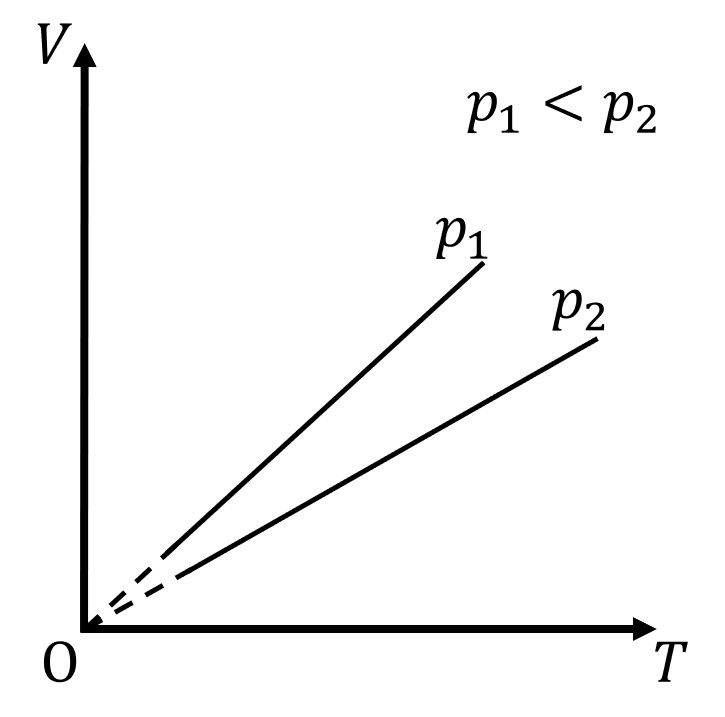
\includegraphics[scale=0.3]{../figs/VN10-PH-39-L-0291-1.jpg}
		\end{center}
	}
	\item \mkstar{2} [8]
	
	\cauhoi{
		Một xi lanh có một pit-tông có thể di chuyển dễ dàng. Ban đầu xi lanh chứa không khí có thể tích $\SI{6}{l}$ ở nhiệt độ $\SI{27}{\celsius}$. Tính thể tích của khí trong xi lanh khi đun nóng đẳng áp đến nhiệt độ $\SI{500}{K}$. Vẽ đồ thị trong hệ tọa độ $\text{O}VT$.
	}
	
	\loigiai{
		Đẳng áp (1): $V_1=\SI{6}{l}$, $T_1=\SI{300}{K}$ sang (2): $V_2=?$, $T_2=\SI{500}{K}$
		
		Vì quá trình là đẳng áp nên ta có phương trình:
		
		$$\dfrac{V_1}{T_1} = \dfrac{V_2}{T_2} \Rightarrow V_2 =\dfrac{V_1T_2}{T_1} = \SI{10}{l}.$$
		
		Đồ thị:
		\begin{center}
			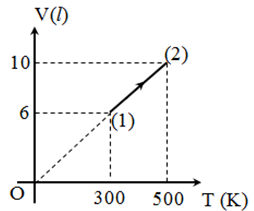
\includegraphics{../figs/VN10-2021-PH-TP032-1}
		\end{center}
	}




\end{enumerate}
\section{Lý thuyết: Phương trình trạng thái của khí lí tưởng}
\begin{enumerate}[label=\bfseries Câu \arabic*:]
	
	\item \mkstar{1} [24]
	
	\cauhoi{
		Ba thông số xác định trạng thái của một lượng khí xác định là
		\begin{mcq}(2)
			\item áp suất, thể tích và khối lượng. 
			\item áp suất, nhiệt độ và khối lượng.
			\item thể tích, trọng lượng và áp suất.
			\item áp suất, nhiệt độ và thể tích.
		\end{mcq}
	}
	
	\loigiai{
		\textbf{Đáp án: D.}
		
		Ba thông số xác định trạng thái của một lượng khí xác định là áp suất, nhiệt độ và thể tích.
	}

\item \mkstar{2} [24]

\cauhoi{
	Ở kì nén của một động cơ đốt trong 4 kì, nhiệt độ của hỗn hợp khí tăng từ $\SI{47}{\celsius}$ đến $\SI{367}{\celsius}$, còn thể tích của khí giảm từ $\SI{1.8}{l}$ xuống còn $\SI{0.3}{l}$. Áp suất của khí lúc bắt đầu nén là $\SI{1}{atm}$. Coi hỗn hợp khí như chất khí lí tưởng. Áp suất khí cuối kì nén là
	\begin{mcq}(4)
		\item $\SI{24}{atm}$. 
		\item $\SI{12}{atm}$.
		\item $\SI{6}{atm}$.
		\item $\SI{2}{atm}$.
	\end{mcq}
}

\loigiai{
	\textbf{Đáp án: B.}
	
	Biến đổi trạng thái (1): $p_1=\SI{1}{atm}$, $V_1=\SI{1.8}{l}$, $T_1=\SI{320}{K}$ sang (2): $p_2=?$, $V_2=\SI{0.3}{l}$, $T_2=\SI{640}{K}$.
	
	Áp dụng phương trình trạng thái khí lí tưởng:
	
	$$\dfrac{p_1V_1}{T_1} = \dfrac{p_2V_2}{T_2} \Rightarrow p_2 =\dfrac{p_1V_1T_2}{T_1V_2} = \SI{12}{atm}.$$
}


\item \mkstar{2} [29]

\cauhoi{
	Một cái bơm chứa $\SI{120}{cm^3}$ không khí ở nhiệt độ $\SI{25}{\celsius}$ và áp suất $\SI{e5}{Pa}$. Áp suất của không khí trong bơm khi lượng khí bị nén xuống còn $\SI{80}{cm^3}$ và nhiệt độ tăng lên tới $\SI{37}{\celsius}$ có giá trị xấp xỉ bằng bao nhiêu?
	\begin{mcq}(4)
		\item $\SI{2.5e5}{Pa}$. 
		\item $\SI{2.0e5}{Pa}$.
		\item $\SI{1.56e5}{Pa}$.
		\item $\SI{1.29e5}{Pa}$.
	\end{mcq}
}

\loigiai{
	\textbf{Đáp án: C.}
	
	Biến đổi trạng thái (1): $p_1=\SI{e5}{Pa}$, $V_1=\SI{120}{cm^3}$, $T_1=\SI{298}{K}$ sang (2): $p_2=?$, $V_2=\SI{80}{cm^3}$, $T_2=\SI{310}{K}$.
	
	Áp dụng phương trình trạng thái khí lí tưởng:
	
	$$\dfrac{p_1V_1}{T_1} = \dfrac{p_2V_2}{T_2} \Rightarrow p_2 =\dfrac{p_1V_1T_2}{T_1V_2} = \SI{1.56e5}{Pa}.$$
}
\item \mkstar{1} [16]

\cauhoi{
	Viết phương trình trạng thái khí lí tưởng, từ đó suy ra công thức tính áp suất ban đầu và thể tích lúc sau.
	
}
\loigiai{
	
	Phương trình trạng thái khí lí tưởng:
	$$\dfrac{p_1V_1}{T_1} = \dfrac{p_2V_2}{T_2}.$$
	
	Suy ra công thức tính áp suất ban đầu:
	$$p_1 = \dfrac{p_2V_2T_1}{T_2V_1}.$$
	
	Suy ra công thức tính thể tích lúc sau:
	$$V_2 = \dfrac{p_1V_1T_2}{T_1p_2}.$$
}
\item \mkstar{2} [4]

\cauhoi{
	Một bình kín có thể tích $\SI{0.4}{m^3}$, chứa khí ở $\SI{27}{\celsius}$ và áp suất $\SI{1.5}{atm}$. Khi mở nắp, áp suất khí còn $\SI{1}{atm}$, nhiệt độ còn $\SI{0}{\celsius}$. Tính thể tích khí thoát ra khỏi bình.
}
\loigiai{
	
	Biến đổi trạng thái (1): $p_1=\SI{1.5}{atm}$, $V_1=\SI{0.4}{m^3}$, $T_1=\SI{300}{K}$ sang (2): $p_2=\SI{1}{atm}$, $V_2=?$, $T_2=\SI{273}{K}$.
	
	Áp dụng phương trình trạng thái:
	
	$$\dfrac{p_1V_1}{T_1} = \dfrac{p_2V_2}{T_2} \Rightarrow V_2 =\dfrac{p_1V_1T_2}{p_2T_1} = \SI{0.546}{m^3}.$$
	
	Vậy thể tích khí thoát ra khỏi bình là $\Delta V = V_2-V_1=\SI{0.146}{m^3}$.
}
\item \mkstar{2} [10]

\cauhoi{
	Một lượng khí ở nhiệt độ $\SI{27}{\celsius}$, thể tích 5 lít và áp suất là $\SI{3}{atm}$. Làm nóng khối khí lên đến nhiệt độ $t_2$ thì thể tích lên đến 8 lít và áp suất là $\SI{2}{atm}$. Tính nhiệt độ $t_2$.
}
\loigiai{
	Biến đổi trạng thái (1): $p_1=\SI{3}{atm}$, $V_1=\SI{5}{l}$, $T_1=\SI{300}{K}$ sang (2): $p_2=\SI{2}{atm}$, $V_2=\SI{8}{l}$, $T_2=?$.
	
	Áp dụng phương trình trạng thái:
	
	$$\dfrac{p_1V_1}{T_1} = \dfrac{p_2V_2}{T_2} \Rightarrow T_2 =\dfrac{p_2V_2T_1}{p_1V_1} = \SI{320}{K}.$$
	
	Đổi $t_2=T_2-273 = \SI{47}{\celsius}$.
}
\item \mkstar{2} [11]

\cauhoi{
	Một lượng khí lí tưởng ở nhiệt độ $\SI{27}{\celsius}$, áp suất $\SI{e5}{Pa}$, thể tích 4 lít được biến đổi trạng thái qua 2 giai đoạn: nén đẳng nhiệt đến áp suất là $\SI{2e5}{Pa}$, sau đó cho dãn nở đẳng áp đến thể tích $\SI{6}{l}$. Xác định các thông số $V_2$, $p_3$.
}
\loigiai{
	
	Đẳng nhiệt (1): $p_1=\SI{e5}{Pa}$, $V_1=\SI{4}{l}$, $T_1=\SI{300}{K}$ sang (2): $p_2=\SI{2e5}{Pa}$, $V_2=?$, $T_2=T_1=\SI{300}{K}$.
	
	Áp dụng phương trình trạng thái:
	
	$$\dfrac{p_1V_1}{T_1} = \dfrac{p_2V_2}{T_2} \Rightarrow V_2 =\dfrac{p_1V_1T_2}{p_2T_1}=\dfrac{p_1V_1}{p_2} = \SI{2}{l}.$$
	
	Đẳng áp (2): $p_2=\SI{2e5}{Pa}$ sang (3): $p_3=p_2=\SI{2e5}{Pa}$.
	
	Vậy $p_3=\SI{2e5}{Pa}$.
}
\item \mkstar{2} [12]

\cauhoi{
	Một khối khí lí tưởng có nhiệt độ $\SI{27}{\celsius}$ ở trạng thái (1). Khí được biến đổi qua hai quá trình:
	\begin{itemize}
		\item Từ trạng thái (1), khí được biến đổi đẳng tích sang trạng thái (2) có áp suất $\SI{1.5}{atm}$ và nhiệt độ là $\SI{177}{\celsius}$, thể tích 10 lít.
		\item Từ trạng thái (2), khí được biến đổi đẳng áp sang trạng thái (3) có nhiệt độ $\SI{627}{\celsius}$.
	\end{itemize}
	Xác định các thông số của từng trạng thái.
}
\loigiai{
	Đẳng tích (1): $p_1=?$, $V_1=\SI{10}{l}$, $T_1=\SI{300}{K}$ sang (2): $p_2=\SI{1.5}{atm}$, $V_2=V_1=\SI{10}{l}$, $T_2=T_1=\SI{450}{K}$.
	
	Áp dụng phương trình trạng thái:
	
	$$\dfrac{p_1V_1}{T_1} = \dfrac{p_2V_2}{T_2} \Rightarrow p_1 =\dfrac{p_2V_2T_1}{V_1T_2}=\dfrac{p_2T_1}{T_2} = \SI{1}{atm}.$$
	
	Đẳng áp (2): $p_2=\SI{1.5}{atm}$, $V_2=\SI{10}{l}$, $T_2=\SI{450}{K}$ sang (3): $p_3=p_2=\SI{1.5}{atm}$, $V_3=?$, $T_3=\SI{900}{K}$.
	
	Áp dụng phương trình trạng thái:
	
	$$\dfrac{p_2V_2}{T_2} = \dfrac{p_3V_3}{T_3} \Rightarrow V_3 =\dfrac{p_2V_2T_3}{T_2p_3}=\dfrac{V_2T_3}{T_2} = \SI{20}{l}.$$
	
}
\item \mkstar{2} [15]

\cauhoi{
	Nhiệt độ ban đầu của hỗn hợp khí trong xi lanh là $T_1$, áp suất $\SI{100}{kPa}$. Nén cho thể tích khí giảm từ $\SI{1.6}{l}$ xuống đến $\SI{0.8}{l}$ thì áp suất tăng thêm $\SI{400}{kPa}$, nhiệt độ tăng thêm $\SI{450}{\celsius}$. Coi hỗn hợp khí là một chất khí thuần nhất. Tính nhiệt độ $T_1$ của khí.
	
}
\loigiai{
	
	Biến đổi trạng thái (1): $p_1=\SI{100}{kPa}$, $V_1=\SI{1.6}{l}$, $T_1$ sang (2): $p_2=p_1+\SI{400}{kPa} = \SI{500}{kPa}$, $V_2=\SI{0.8}{l}$, $T_2=T_1+\SI{450}{\celsius} = T_1 + \SI{450}{K}$.
	
	Áp dụng phương trình trạng thái khí lí tưởng:
	
	$$\dfrac{p_1V_1}{T_1} = \dfrac{p_2V_2}{T_2} \Rightarrow T_1 = \dfrac{p_1V_1T_2}{p_2V_2}=\dfrac{p_1V_2(T_1+450)}{p_2V_2} \Rightarrow T_1 = \SI{300}{K}.$$
}



\item \mkstar{2} [16]

\cauhoi{
	Một lượng khí đựng trong một xi lanh có pit-tông chuyển động được. Trạng thái của lượng khí lúc đầu là $\SI{2}{atm}$, $\SI{15}{l}$, $\SI{27}{\celsius}$. Khi pit-tông nén khí, áp suất của khí tăng lên tới $\SI{3.5}{atm}$, thể tích giảm còn $\SI{12}{l}$. Xác định nhiệt độ của khí sau khi nén.
	
}
\loigiai{
	
	Biến đổi trạng thái (1): $p_1=\SI{2}{atm}$, $V_1=\SI{15}{l}$, $T_1=\SI{300}{K}$ sang (2): $p_2=\SI{3.5}{atm}$, $V_2=\SI{12}{l}$, $T_2=?$.
	
	Áp dụng phương trình trạng thái khí lí tưởng:
	
	$$\dfrac{p_1V_1}{T_1} = \dfrac{p_2V_2}{T_2} \Rightarrow T_2 =\dfrac{p_2V_2T_1}{p_1V_1} = \SI{420}{K}.$$
	
	Đổi $t_2=T_2-273 = \SI{147}{\celsius}$.
}

\item \mkstar{2} [17]

\cauhoi{
	Một quả "bóng thám không" có thể tích 300 lít ở nhiệt độ $\SI{27}{\celsius}$ và áp suất $\SI{e5}{Pa}$ trên mặt đất. Bóng được thả ra và bay lên đến độ cao mà ở đó áp suất chỉ còn $\SI{0.5e5}{Pa}$ và nhiệt độ lúc này là $\SI{7}{\celsius}$. Tính thể tích của quả bóng ở độ cao đó.
	
}
\loigiai{
	Biến đổi trạng thái (1): $p_1=\SI{e5}{Pa}$, $V_1=\SI{300}{l}$, $T_1=\SI{300}{K}$ sang (2): $p_2=\SI{0.5e5}{Pa}$, $V_2=?$, $T_2=\SI{280}{K}$.
	
	Áp dụng phương trình trạng thái khí lí tưởng:
	
	$$\dfrac{p_1V_1}{T_1} = \dfrac{p_2V_2}{T_2} \Rightarrow V_2 =\dfrac{p_1V_1T_2}{T_1p_2} = \SI{560}{l}.$$
}
\item \mkstar{2} [18]

\cauhoi{
	Ở kì nén của một động cơ đốt trong 4 kì, nhiệt độ của hỗn hợp khí tăng từ $\SI{47}{\celsius}$ đến $\SI{367}{\celsius}$, còn thể tích của khí giảm từ $\SI{1.8}{l}$ còn $\SI{0.3}{l}$. Áp suất của khí lúc bắt đầu nén là $\SI{150}{kPa}$. Coi hỗn hợp khí như chất khí thuần nhất, áp suất cuối kì nén là bao nhiêu kPa?
	
}
\loigiai{
	
	Biến đổi trạng thái (1): $p_1=\SI{150}{kPa}$, $V_1=\SI{1.8}{l}$, $T_1=\SI{320}{K}$ sang (2): $p_2=?$, $V_2=\SI{0.3}{l}$, $T_2=\SI{640}{K}$.
	
	Áp dụng phương trình trạng thái khí lí tưởng:
	
	$$\dfrac{p_1V_1}{T_1} = \dfrac{p_2V_2}{T_2} \Rightarrow p_2 =\dfrac{p_1V_1T_2}{T_1V_2} = \SI{1800}{kPa}.$$
}
	\item \mkstar{3} [1]
	
	\cauhoi{
		\begin{enumerate}[label=\alph*)]
			\item Kể tên các đại lượng đặc trưng cho trạng thái của một lượng khí. Viết biểu thức liên hệ giữa các đại lượng này.
			\item Trong xi lanh của một động cơ đốt trong, bên dưới pit-tông có chứa hỗn hợp khí ở nhiệt độ $\SI{47}{\celsius}$. Sau đó, nén pit-tông làm cho thể tích của hỗn hợp khí giảm 10 lần thì áp suất tăng gấp 15 lần. Hãy tính nhiệt độ của hỗn hợp khí sau khi bị nén (theo đơn vị độ C). Hỗn hợp khí được xem là khí lí tưởng.
		\end{enumerate}
	}
	\loigiai{
		
		\begin{enumerate}[label=\alph*)]
			\item Các đại lượng đặc trưng cho trạng thái của một lượng khí: áp suất, thể tích, nhiệt độ (tuyệt đối). Biểu thức liên hệ: $\dfrac{pV}{T} = \text{hằng số}$ hay $\dfrac{p_1V_1}{T_1} = \dfrac{p_2V_2}{T_2}$.
			
			\item Biến đổi trạng thái (1): $p_1$, $V_1$, $T_1=\SI{320}{K}$ sang (2): $p_2=15p_1$, $V_2=\dfrac{V_1}{10}$, $T_2=?$.
			
			Áp dụng phương trình trạng thái khí lí tưởng:
			
			$$\dfrac{p_1V_1}{T_1} = \dfrac{p_2V_2}{T_2} \Rightarrow T_2 =\dfrac{p_2V_2T_1}{p_1V_1} = \SI{480}{K}.$$
			
			Đổi $t_2=T_2-273=\SI{207}{\celsius}$.
		\end{enumerate}
	}
\item \mkstar{3} [1]

\cauhoi{
	Một khối khí lí tưởng ở trạng thái ban đầu có áp suất $p_1=\SI{6}{atm}$, thể tích $V_1=\SI{2}{l}$ và nhiệt độ $t_1=\SI{27}{\celsius}$ biến đổi lần lượt qua các quá trình:
	\begin{itemize}
		\item Đẳng áp sang trạng thái 2 có nhiệt độ $t_2=\SI{627}{\celsius}$;
		\item Đẳng tích sang trạng thái 3 có áp suất $p_3=\SI{2}{atm}$;
		\item Đẳng nhiệt sang trạng thái 4 có thể tích $V_4=\SI{3}{l}$.
	\end{itemize}
	Tìm nhiệt độ ở trạng thái 3 và áp suất sau cùng của khối khí.
}
\loigiai{
	
	\begin{itemize}
		\item Đẳng áp (1): $p_1=\SI{6}{atm}$, $V_1=\SI{2}{l}$, $T_1=\SI{300}{K}$ sang (2): $p_2=p_1=\SI{6}{atm}$, $V_2=?$, $T_2=\SI{900}{K}$.
		
		Áp dụng phương trình trạng thái:
		
		$$\dfrac{p_1V_1}{T_1} = \dfrac{p_2V_2}{T_2} \Rightarrow V_2 =\dfrac{p_1V_1T_2}{p_2T_1} = \dfrac{V_1T_2}{T_1} = \SI{6}{l}.$$
		
		
		\item Đẳng tích (2): $p_2=\SI{6}{atm}$, $V_2=\SI{6}{l}$, $T_2=\SI{900}{K}$ sang (3): $p_3=\SI{2}{atm}$, $V_3=V_2=\SI{6}{l}$, $T_3=?$.
		
		Áp dụng phương trình trạng thái:
		
		$$\dfrac{p_2V_2}{T_2} = \dfrac{p_3V_3}{T_3} \Rightarrow T_3 =\dfrac{p_3V_3T_2}{p_2V_2}=\dfrac{p_3T_2}{p_2} =  \SI{300}{K}.$$
		
		
		\item Đẳng nhiệt (3): $p_3=\SI{2}{atm}$, $V_3=\SI{6}{l}$, $T_3=\SI{300}{K}$ sang (4): $p_4=?$, $V_4=\SI{3}{l}$, $T_4=T_3=\SI{300}{K}$.
		
		Áp dụng phương trình trạng thái:
		
		$$\dfrac{p_3V_3}{T_3} = \dfrac{p_4V_4}{T_4} \Rightarrow p_4 =\dfrac{p_3V_3T_4}{V_4T_3} = \dfrac{p_3V_3}{V_4} = \SI{4}{atm}.$$
		
		
	\end{itemize}
}
\item \mkstar{3} [14]

\cauhoi{
	Khi cho một lượng khí xác định được nén đẳng nhiệt từ thể tích $V_1=V_0$ sang thể tích $V_2=\dfrac{1}{3}V_0$ thì nhận thấy áp suất của lượng khí tăng thêm một lượng $\SI{2}{atm}$. Sau đó tiếp tục đun nóng đẳng tích đến khi nhiệt độ của khối khí tăng thêm $\SI{100}{\celsius}$ thì áp suất khối khí lúc này là $\SI{8}{atm}$. Xác định nhiệt độ ban đầu của lượng khí.
}
\loigiai{
	
	Đẳng nhiệt (1): $p_1$, $V_1=V_0$, $T_1=?$ sang (2): $p_2=p_1 + \SI{2}{atm}$, $V_2=\dfrac{V_0}{3}$, $T_2=T_1$.
	
	Áp dụng phương trình trạng thái:
	
	$$\dfrac{p_1V_1}{T_1} = \dfrac{p_2V_2}{T_2} \Rightarrow p_1V_1 = p_2V_2 \Rightarrow p_1 V_0 = (p_1+2) \dfrac{1}{3}V_0 \Rightarrow p_1=\SI{1}{atm}. $$
	
	Đẳng tích (2): $p_2=p_1+\SI{2}{atm}$, $V_2=\dfrac{1}{3}V_0$, $T_2=T_1$ sang (3): $p_3=\SI{8}{atm}$, $V_3=V_2=\dfrac{1}{3}V_0$, $T_3=T_2+\SI{100}{\celsius} = T_1 + \SI{100}{K}$.
	
	Áp dụng phương trình trạng thái:
	
	$$\dfrac{p_2V_2}{T_2} = \dfrac{p_3V_3}{T_3} \Rightarrow \dfrac{p_1+2}{T_1} = \dfrac{8}{T_1+100} \Rightarrow T_1 = \SI{60}{K}.$$
}
\item \mkstar{3} [20]

\cauhoi{
	Một khối khí lí tưởng có thể tích $\SI{10}{l}$, nhiệt độ $\SI{27}{\celsius}$, áp suất $\SI{2}{atm}$. Khối khí này biến đổi qua hai quá trình:
	\begin{itemize}
		\item đẳng nhiệt: áp suất tăng gấp đôi.
		\item đẳng áp: nhiệt độ sau cùng là $\SI{327}{\celsius}$.
	\end{itemize}
	Tìm các thông số trạng thái chưa biết.
}
\loigiai{
	
	Đẳng nhiệt (1): $p_1=\SI{2}{atm}$, $V_1=\SI{10}{l}$, $T_1=\SI{300}{K}$ sang (2): $p_2=2p_1 = \SI{4}{atm}$, $V_2=?$, $T_2=T_1=\SI{300}{K}$.
	
	Áp dụng phương trình trạng thái:
	
	$$\dfrac{p_1V_1}{T_1} = \dfrac{p_2V_2}{T_2} \Rightarrow V_2 = \dfrac{p_1V_1T_2}{p_2T_1} = \dfrac{p_1V_1}{p_2} =\SI{5}{l}.$$
	
	Đẳng áp (2): $p_2=\SI{4}{atm}$, $V_2=\SI{5}{l}$, $T_2=\SI{300}{K}$ sang (3): $p_3=p_2=\SI{4}{atm}$, $V_3=?$, $T_3=\SI{600}{\celsius}$.
	
	Áp dụng phương trình trạng thái:
	
	$$\dfrac{p_2V_2}{T_2} = \dfrac{p_3V_3}{T_3} \Rightarrow V_3= \dfrac{p_2V_2T_3}{T_2p_3}=\dfrac{V_2T_3}{T_2}= \SI{10}{l}.$$
}

\item \mkstar{3} [21]

\cauhoi{
	Một khối khí lí tưởng có áp suất ban đầu $p_1$, thể tích 3 lít ở nhiệt độ $\SI{27}{\celsius}$ được biến đổi trạng thái qua hai quá trình liên tiếp nhau:
	\begin{itemize}
		\item Quá trình 1: làm lạnh đẳng tích để áp suất bằng $3/4$ áp suất ban đầu;
		\item Quá trình 2: nén đẳng nhiệt đến áp suất bằng $1/2$ áp suất ban đầu.
	\end{itemize}
	\begin{enumerate}[label=\alph*)]
		\item Tính nhiệt độ khí ở trạng thái (2) theo độ C.
		\item Tính thể tích khí ở trạng thái (3).
	\end{enumerate}
	
}
\loigiai{
	\begin{enumerate}[label=\alph*)]
		\item Tính nhiệt độ khí ở trạng thái (2) theo độ C.
		Đẳng tích (1): $p_1$, $V_1=\SI{3}{l}$, $T_1=\SI{300}{K}$ sang (2): $p_2=\dfrac{3}{4}p_1$, $V_2=V_1=\SI{3}{l}$, $T_2=?$.
		
		Áp dụng phương trình trạng thái:
		
		$$\dfrac{p_1V_1}{T_1} = \dfrac{p_2V_2}{T_2} \Rightarrow T_2=\dfrac{p_2V_2T_1}{p_1V_1} = \dfrac{p_2T_1}{p_1}=\SI{225}{K}.$$
		
		Đổi $t_2 = T_2 - 273 = \SI{-48}{\celsius}$.
		
		\item Tính thể tích khí ở trạng thái (3).
		Đẳng nhiệt (2): $p_2=\dfrac{3}{4}p_1$, $V_2=\SI{3}{l}$, $T_2=\SI{225}{K}$ sang (3): $p_3=\dfrac{1}{2}p_1$, $V_3=?$, $T_3=T_2$.
		
		Áp dụng phương trình trạng thái:
		
		$$\dfrac{p_2V_2}{T_2} = \dfrac{p_3V_3}{T_3} \Rightarrow V_3 = \dfrac{p_2V_2T_3}{p_3T_2} = \dfrac{p_2V_2}{p_3} = \SI{4.5}{l}.$$
	\end{enumerate}
}

\item \mkstar{3} [22]

\cauhoi{
	Một khối khí lí tưởng có áp suất ban đầu $\SI{1.5}{atm}$, thể tích 10 lít ở nhiệt độ $\SI{87}{\celsius}$ được biến đổi trạng thái qua hai quá trình liên tiếp nhau:
	\begin{itemize}
		\item Quá trình 1: đẳng áp, nhiệt độ tuyệt đối giảm 2 lần;
		\item Quá trình 2: đẳng nhiệt, áp suất sau cùng là $\SI{1}{atm}$.
	\end{itemize}
	\begin{enumerate}[label=\alph*)]
		\item Tìm thể tích $V_2$ của khối khí sau quá trình 1.
		\item Tìm thể tích $V_3$ của khối khí sau quá trình 2.
	\end{enumerate}
	
}
\loigiai{
	\begin{enumerate}[label=\alph*)]
		\item Tìm thể tích $V_2$ của khối khí sau quá trình 1.
		Đẳng áp (1): $p_1=\SI{1.5}{atm}$, $V_1=\SI{10}{l}$, $T_1=\SI{360}{K}$ sang (2): $p_2=p_1=\SI{1.5}{atm}$, $V_2=?$, $T_2=\dfrac{T_1}{2} = \SI{180}{K}$.
		
		Áp dụng phương trình trạng thái:
		
		$$\dfrac{p_1V_1}{T_1} = \dfrac{p_2V_2}{T_2} \Rightarrow V_2=\dfrac{p_1V_1T_2}{p_2T_1} = \dfrac{V_1T_2}{T_1}=\SI{5}{l}.$$
		
		\item Tìm thể tích $V_3$ của khối khí sau quá trình 2.
		Đẳng nhiệt (2): $p_2=\SI{1.5}{atm}$, $V_2=\SI{5}{l}$, $T_2=\SI{180}{K}$ sang (3): $p_3=\SI{1}{atm}$, $V_3=?$, $T_3=T_2=\SI{180}{K}$.
		
		Áp dụng phương trình trạng thái:
		
		$$\dfrac{p_2V_2}{T_2} = \dfrac{p_3V_3}{T_3} \Rightarrow V_3 = \dfrac{p_2V_2T_3}{p_3T_2} = \dfrac{p_2V_2}{p_3} = \SI{7.5}{l}.$$
	\end{enumerate}
}

\item \mkstar{3} [23]

\cauhoi{
	Một lượng khí lí tưởng có áp suất $p_1=\SI{1}{atm}$, nhiệt độ $t_1=\SI{27}{\celsius}$ và thể tích $V_1=\SI{1}{l}$ biến đổi lần lượt qua hai quá trình sau:
	\begin{itemize}
		\item Biến đổi đẳng nhiệt tới thể tích $V_2=\SI{2}{l}$, áp suất $p_2$;
		\item Biến đổi đẳng tích tới áp suất $p_3=2p_2$, nhiệt độ $t_3$.
	\end{itemize}
	Tìm $p_2$, $t_3$.
}
\loigiai{
	Đẳng nhiệt (1): $p_1=\SI{1}{atm}$, $V_1=\SI{1}{l}$, $T_1=\SI{300}{K}$ sang (2): $p_2=?$, $V_2=\SI{2}{l}$, $T_2=T_1 = \SI{300}{K}$.
	
	Áp dụng phương trình trạng thái:
	
	$$\dfrac{p_1V_1}{T_1} = \dfrac{p_2V_2}{T_2} \Rightarrow p_2=\dfrac{p_1V_1T_2}{V_2T_1} = \dfrac{p_1V_1}{V_2}=\SI{0.5}{atm}.$$
	
	Đẳng tích (2): $p_2=\SI{0.5}{atm}$, $V_2=\SI{2}{l}$, $T_2=\SI{300}{K}$ sang (3): $p_3=2p_2=\SI{1}{atm}$, $V_3=V_2=\SI{2}{l}$, $T_3=?$.
	
	Áp dụng phương trình trạng thái:
	
	$$\dfrac{p_2V_2}{T_2} = \dfrac{p_3V_3}{T_3} \Rightarrow T_3=\dfrac{p_3V_3T_2}{p_2V_2} = \dfrac{p_3T_2}{p_2}=\SI{600}{K}.$$
	
	Đổi $t_3=T_3-273=\SI{327}{\celsius}$.
}
\item \mkstar{3} [26]

\cauhoi{
	Một khối khí lí tưởng có thể tích 5 lít, ở nhiệt độ $\SI{227}{\celsius}$ và áp suất $\SI{1}{atm}$. Cho khối khí biến đổi qua 2 quá trình liên tiếp nhau:
	\begin{itemize}
		\item Quá trình 1: làm lạnh đẳng áp cho thể tích giảm còn phân nửa thể tích ban đầu;
		\item Quá trình 2: nung nóng đẳng tích để áp suất tăng lên thêm một lượng bằng $1/2$ áp suất ban đầu.
	\end{itemize}
	Tính nhiệt độ của khối khí ở cuối mỗi quá trình ra độ C.
}
\loigiai{
	Đẳng áp (1): $p_1=\SI{1}{atm}$, $V_1=\SI{5}{l}$, $T_1=\SI{500}{K}$ sang (2): $p_2=p_1=\SI{1}{atm}$, $V_2=\dfrac{V_1}{2}=\SI{2.5}{l}$, $T_2=?$.
	
	Áp dụng phương trình trạng thái:
	
	$$\dfrac{p_1V_1}{T_1} = \dfrac{p_2V_2}{T_2} \Rightarrow T_2=\dfrac{p_2V_2T_1}{p_1V_1} = \dfrac{V_2T_1}{V_1}=\SI{250}{K}.$$
	
	Đổi $t_2=T_2-273=\SI{-23}{\celsius}$
	
	Đẳng tích (2): $p_2=\SI{1}{atm}$, $V_2=\SI{2.5}{l}$, $T_2=\SI{250}{K}$ sang (3): $p_3=1,5p_1=\SI{1.5}{atm}$, $V_3=V_2=\SI{2.5}{l}$, $T_3=?$.
	
	Áp dụng phương trình trạng thái:
	
	$$\dfrac{p_2V_2}{T_2} = \dfrac{p_3V_3}{T_3} \Rightarrow T_3=\dfrac{p_3V_3T_2}{p_2V_2} = \dfrac{p_3T_2}{p_2}=\SI{375}{K}.$$
	
	Đổi $t_3=T_3-273=\SI{102}{\celsius}$.
}
\item \mkstar{3} [29]

\cauhoi{
	Tính nhiệt độ tuyệt đối ban đầu của một khối khí xác định, biết rằng khi nhiệt độ tăng thêm $\SI{16}{\celsius}$ thì thể tích giảm đi $10\%$, còn áp suất thì tăng thêm $20\%$ so với ban đầu.
}

\loigiai{
	
	Biến đổi trạng thái (1): $p_1$, $V_1$, $T_1$ sang (2): $p_2=(1+0,2)p_1$, $V_2=(1-0,1)V_1$, $T_2=T_1+\SI{16}{\celsius}$.
	
	Áp dụng phương trình trạng thái khí lí tưởng:
	
	$$\dfrac{p_1V_1}{T_1} = \dfrac{p_2V_2}{T_2} \Rightarrow T_1 = \SI{200}{K}.$$
}
\item \mkstar{4} [3]

\cauhoi{
	
	Khối lượng riêng của không khí xác định bởi công thức $D=\dfrac{m}{V}$ (với $m$ là khối lượng không khí ứng với thể tích $V$). Ở điều kiện tiêu chuẩn ($\SI{0}{\celsius}$, $\SI{760}{mmHg}$) thì khối lượng riêng của không khí là $D_0=\SI{1.29}{kg/m^3}$. Tính khối lượng không khí chứa trong một căn phòng có thể tích $\SI{55}{m^3}$ ở vùng cao nguyên có nhiệt độ $\SI{17}{\celsius}$, áp suất $\SI{660}{mmHg}$.
}
\loigiai{
	
	Biến đổi trạng thái (1): $p_1=\SI{760}{mmHg}$, $V_1=\dfrac{m}{\SI{1.29}{kg/m^3}}$, $T_1=\SI{273}{K}$ sang (2): $p_2=\SI{660}{mmHg}$, $V_2=\SI{55}{m^3}$, $T_2=\SI{290}{K}$.
	
	Áp dụng phương trình trạng thái:
	
	$$\dfrac{p_1V_1}{T_1} = \dfrac{p_2V_2}{T_2} \Rightarrow m = \SI{58}{kg}.$$
}


	



\item \mkstar{4} [17]

\cauhoi{
	Tính khối lượng riêng của không khí ở đỉnh núi cao $\SI{3220}{m}$. Biết rằng mỗi khi lên cao $\SI{10}{m}$ thì áp suất khí quyển giảm $\SI{1}{mmHg}$ và nhiệt độ trên đỉnh núi là $\SI{2}{\celsius}$. Khối lượng riêng của không khí ở điều kiện chuẩn (áp suất $\SI{760}{mmHg}$ và nhiệt độ $\SI{0}{\celsius}$) là $\SI{1.29}{kg/m^3}$.
}
\loigiai{
	
	Áp suất trên đỉnh núi:
	$$p_2 = p_1 - \dfrac{\SI{3220}{m}}{\SI{10}{m}} \cdot \SI{1}{mmHg} = p_1 - \SI{322}{mmHg} = \SI{760}{mmHg} - \SI{322}{mmHg} = \SI{438}{mmHg}.$$
	
	Vì $m_1 = m_2$ nên $V_1D_1 = V_2D_2$, áp dụng phương trình trạng thái:
	$$\dfrac{p_1V_1}{T_1} = \dfrac{p_2V_2}{T_2} \Rightarrow \dfrac{p_1}{D_1 T_1} = \dfrac{p_2}{D_2 T_2} \Rightarrow D_2 = \SI{0.74}{kg/m^3}.$$
}





\item \mkstar{4} [23]

\cauhoi{
	Có hai bình cầu nối với nhau bằng một ống dẫn có khóa. Bình thứ nhất có dung tích $V_1=\SI{15}{l}$ chứa khí có áp suất $p_1=\SI{2e5}{Pa}$. Bình thứ hai có dung tích $V_2=\SI{5}{l}$. Mở khóa nhẹ nhàng để hai bình thông nhau sao cho nhiệt độ của hai bình luôn bằng nhiệt độ phòng. Biết thể tích của ống dẫn là nhỏ và có thể bỏ qua. Tính áp suất trong hai bình khi đã cân bằng. Xét hai trường hợp sau:
	\begin{enumerate}[label=\alph*)]
		\item Ban đầu bình 2 không chứa khí.
		\item Ban đầu bình 2 chứa khí cùng loại với bình 1, áp suất là $p_2=\SI{1.2e5}{Pa}$.
	\end{enumerate}
	
}
\loigiai{
	Nhiệt độ của hai bình luôn bằng nhiệt độ phòng nên quá trình là đẳng nhiệt.
	\begin{enumerate}[label=\alph*)]
		\item Ban đầu bình 2 không chứa khí.
		
		Khi mở khóa, 15 lít khí trong bình 1 sẽ tràn vào bình 2, làm cho thể tích của toàn bộ lượng khí của hệ tăng từ 15 lít lên đến $V'=\SI{20}{l}$.
		
		Khi cân bằng, áp suất khí trong bình 1 bằng áp suất khí trong bình 2, do đó $p'=p_1' = p_2'$. Áp dụng định luật Bôi-lơ - Ma-ri-ốt cho lượng khí trong toàn bộ hệ:
		$$p_1V_1 = p' V'\Rightarrow p' = \SI{1.5e5}{Pa}.$$
		
		\item Ban đầu bình 2 chứa khí cùng loại với bình 1, áp suất là $p_2=\SI{1.2e5}{Pa}$.
		
		Ta thực hiện phương pháp cô lập từng phần bình, nghĩa là xem như lúc đầu chỉ có bình 1 chứa khí, hoặc chỉ có bình 2 chứa khí. Sau đó cộng áp suất riêng phần của hai bình thì được áp suất khí sau khi cân bằng.
		
		Áp dụng định luật Bôi-lơ - Ma-ri-ốt cho lượng khí trong bình 2, tính được áp suất riêng phần do khí trong bình 2 gây ra lúc sau:
		$$p_2V_2 = p_2'' V_2'' \Rightarrow p_2'' = \dfrac{p_2V_2}{V_2''} = \dfrac{p_2V_2}{V'} = \SI{0.3e5}{Pa}.$$
		
		
		Áp dụng định luật Bôi-lơ - Ma-ri-ốt cho lượng khí trong bình 1, tính được áp suất riêng phần do khí trong bình 1 gây ra lúc sau:
		$$p_1V_1 = p_1'' V_1'' \Rightarrow p_1'' = \dfrac{p_1V_1}{V_1''} = \dfrac{p_1V_1}{V'} = \SI{1.5e5}{Pa}.$$
		
		Áp suất khi cân bằng: $p''=p_1'' + p_2'' = \SI{1.8e5}{Pa}$.
	\end{enumerate}
}

\end{enumerate}

\section{Lý thuyết: Đồ thị biến đổi trạng thái khí lí tưởng}
\begin{enumerate}[label=\bfseries Câu \arabic*:]
	
	\item \mkstar{2} [4]
	
	\cauhoi{
		
			Một lượng khí lí tưởng xác định biến đổi theo chu trình như hình vẽ bên. Nếu chuyển đồ thị sang hệ trục tọa độ $(p,V)$ thì đáp án nào mô tả tương đương?
		
		
		\begin{center}
			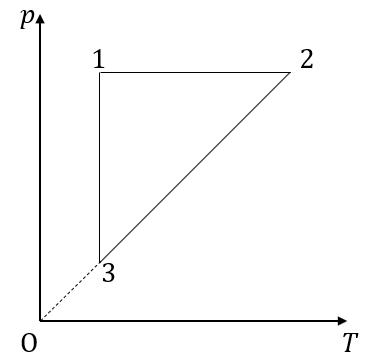
\includegraphics[scale=0.7]{../figs/VN10-2021-PH-TP032-2}
		\end{center}
		\begin{mcq}(2)
			\item 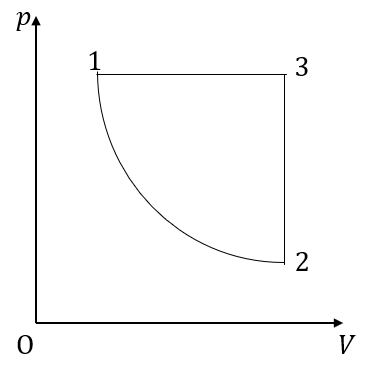
\includegraphics[scale=0.7]{../figs/VN10-2021-PH-TP032-3} 
			\item 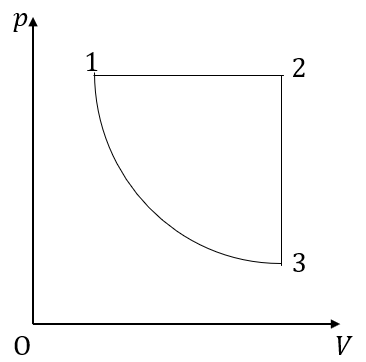
\includegraphics[scale=0.7]{../figs/VN10-2021-PH-TP032-4}
			\item 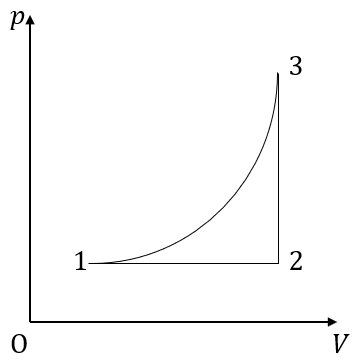
\includegraphics[scale=0.7]{../figs/VN10-2021-PH-TP032-5}
			\item 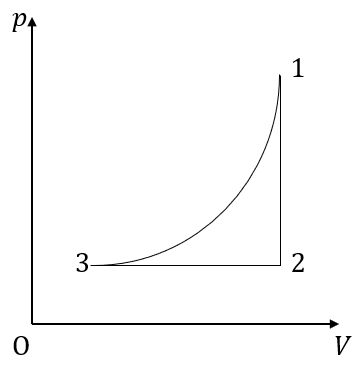
\includegraphics[scale=0.7]{../figs/VN10-2021-PH-TP032-6}
		\end{mcq}
	}
	
	\loigiai{
		\textbf{Đáp án: B.}
		
		Từ (1) sang (2) là quá trình đẳng áp, nhiệt độ tăng;
		
		Từ (2) sang (3) là quá trình đẳng tích, áp suất giảm;
		
		Từ (3) sang (1) là quá trình đẳng nhiệt, áp suất tăng.
	}
\item \mkstar{1} [10]

\cauhoi{
	Các đồ thị sau đây biểu diễn quá trình nào?
	\begin{center}
		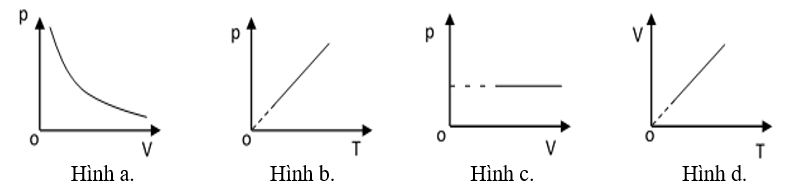
\includegraphics{../figs/VN10-2021-PH-TP032-12}
	\end{center}
}
\loigiai{
	\begin{itemize}
		\item Hình a: đẳng nhiệt;
		\item Hình b: đẳng tích;
		\item Hình c: đẳng áp;
		\item Hình d: đẳng áp.
	\end{itemize}
}
\item \mkstar{1} [13]

\cauhoi{
	Cho đồ thị như hình vẽ. Hãy đọc tên các quá trình biến đổi trạng thái.
	\begin{center}
		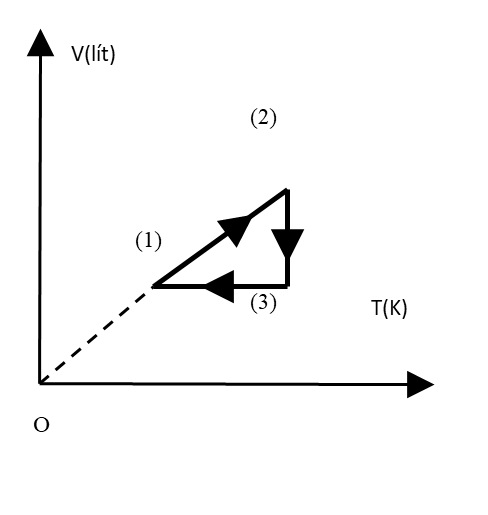
\includegraphics[scale=2]{../figs/VN10-2021-PH-TP032-15}
	\end{center}
	
}
\loigiai{
	Từ (1) sang (2): quá trình đẳng áp;
	
	Từ (2) sang (3): quá trình đẳng nhiệt;
	
	Từ (3) sang (1): quá trình đẳng tích.
}


	\item \mkstar{2} [2]

\cauhoi{
	Hình bên thể hiện quá trình chuyển từ trạng thái (1) sang (2) của một khối khí thì khí bị nén hay giãn? Giải thích.
	\begin{center}
		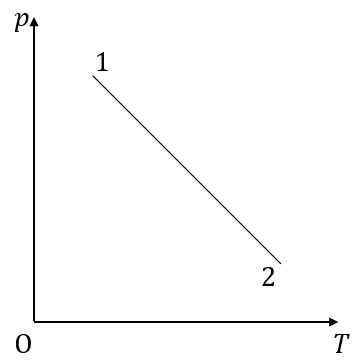
\includegraphics[scale=0.7]{../figs/VN10-2021-PH-TP032-8}
	\end{center}
}

\loigiai{
	
	Trong quá trình từ (1) sang (2) áp suất giảm, nhiệt độ tăng. Ta có $\dfrac{pV}{T} = \text{hằng số} \Rightarrow V \sim \dfrac{T}{p}$. Khi $T$ tăng, $p$ giảm thì $V$ tăng. Khối khí bị giãn.
}

	\item \mkstar{2} [3]

\cauhoi{
	Một khối khí lí tưởng được biến đổi trạng thái theo một chu trình kín như hình vẽ. Cho biết áp suất ban đầu của khối khí $p_1=\SI{9}{atm}$. Tính nhiệt độ $T_1$ và áp suất $p_3$ của khối khí.
	\begin{center}
		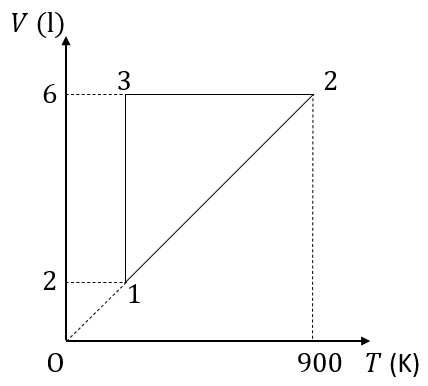
\includegraphics[scale=0.7]{../figs/VN10-2021-PH-TP032-9}
	\end{center}
}

\loigiai{
	Đẳng áp (1): $V_1=\SI{2}{l}$, $T_1=?$ sang (2): $V_2=\SI{6}{l}$, $T_2=\SI{900}{K}$.
	
	Vì quá trình là đẳng áp nên ta có phương trình:
	
	$$\dfrac{V_1}{T_1} = \dfrac{V_2}{T_2} \Rightarrow T_1 =\dfrac{V_1T_2}{V_2} = \SI{300}{K}.$$
	
	Đẳng tích (2): $p_2$, $T_2=\SI{900}{K}$ sang (3): $p_3=?$, $T_3=\SI{300}{K}$.
	
	Vì quá trình là đẳng tích nên ta có phương trình:
	
	$$\dfrac{p_2}{T_2} = \dfrac{p_3}{T_3} \Rightarrow p_2 =\dfrac{p_3T_2}{T_3} = 3p_3.$$
	
	Mà $p_1=p_2=\SI{9}{atm}$ nên $p_3 = \dfrac{p_2}{3} = \SI{3}{atm}$.
	
}

	\item \mkstar{2} [5]

\cauhoi{
	
		Một khối khí thực hiện một chu trình như hình vẽ. Cho $p_1=\SI{5e5}{Pa}$, $V_1=\SI{2.5}{l}$, $T_2=\SI{300}{K}$, $V_2=\SI{6.25}{l}$.
		\begin{enumerate}[label=\alph*)]
			\item Nêu tên gọi các đẳng quá trình trong chu trình.
			\item Tính $p_2$ và $T_3$.
		\end{enumerate}


	\begin{center}
		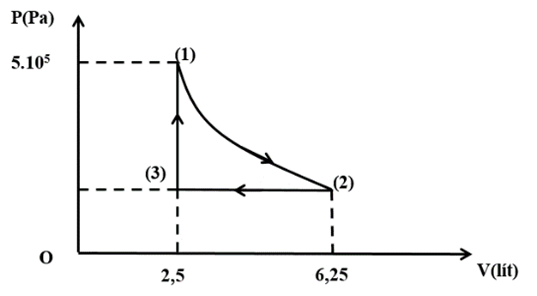
\includegraphics[scale=1.2]{../figs/VN10-2021-PH-TP032-10}
	\end{center}
	
}

\loigiai{
	\begin{enumerate}[label=\alph*)]
		\item Nêu tên gọi các đẳng quá trình trong chu trình.
		
		Từ (1) sang (2): đẳng nhiệt;
		
		Từ (2) sang (3): đẳng áp;
		
		Từ (3) sang (1): đẳng tích.
		
		\item Tính $p_2$ và $T_3$.
		
		Đẳng nhiệt (1): $V_1=\SI{2.5}{l}$, $p_1=\SI{5e5}{Pa}$ sang (2): $p_2=?$, $V_2=\SI{6.25}{l}$.
		
		Vì quá trình là đẳng nhiệt nên ta có phương trình:
		
		$$p_1V_1 = p_2V_2 \Rightarrow p_2 =\dfrac{p_1V_1}{V_2} = \SI{2e5}{Pa}.$$
		
		Đẳng áp (2): $V_2=\SI{6.25}{l}$, $T_2=\SI{300}{K}$ sang (3): $V_3=\SI{2.5}{l}$, $T_3=?$.
		
		Vì quá trình là đẳng áp nên ta có phương trình:
		
		$$\dfrac{V_2}{T_2} = \dfrac{V_3}{T_3} \Rightarrow T_3 =\dfrac{V_3T_2}{V_2} = \SI{120}{K}.$$
		
	\end{enumerate}
}
	
	\item \mkstar{2} [8]
	
	\cauhoi{
		Một khối khí lí tưởng thực hiện các quá trình biến đổi trạng thái theo đồ thị bên.
		\begin{enumerate}[label=\alph*)]
			\item Nêu tên các quá trình biến đổi trạng thái trên đồ thị.
			\item Biết rằng trạng thái 1 có các thông số $V_1=\SI{10}{l}$, $p_1=\SI{2}{atm}$, $T_1=\SI{200}{K}$, trạng thái 2 có áp suất $p_2=\SI{8}{atm}$. Tính thể tích ở trạng thái 2 và nhiệt độ tuyệt đối ở trạng thái 3.
		\end{enumerate}
	\begin{center}
		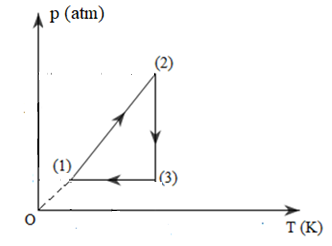
\includegraphics[scale=1.2]{../figs/VN10-2021-PH-TP032-11}
	\end{center}
		
	}
	\loigiai{
		
		\begin{enumerate}[label=\alph*)]
			\item Nêu tên các quá trình biến đổi trạng thái trên đồ thị.
			
			Từ (1) sang (2): đẳng tích;
			
			Từ (2) sang (3): đẳng nhiệt;
			
			Từ (3) sang (1): đẳng áp.
			
			\item Biết rằng trạng thái 1 có các thông số $V_1=\SI{10}{l}$, $p_1=\SI{2}{atm}$, $T_1=\SI{200}{K}$, trạng thái 2 có áp suất $p_2=\SI{8}{atm}$. Tính thể tích ở trạng thái 2 và nhiệt độ tuyệt đối ở trạng thái 3.
			
			Từ (1) sang (2) là đẳng tích nên $V_2=V_1 = \SI{10}{l}$.
			
			Đẳng tích (1): $p_1=\SI{2}{atm}$, $T_1=\SI{200}{K}$ sang (2): $p_2=\SI{8}{atm}$, $T_2=?$.
			
			Vì quá trình là đẳng tích nên ta có phương trình:
			
			$$\dfrac{p_1}{T_1} = \dfrac{p_2}{T_2} \Rightarrow T_2 =\dfrac{p_2T_1}{p_1} = \SI{800}{K}.$$
			
			Từ (2) sang (3) là đẳng nhiệt nên $T_3=T_2=\SI{800}{K}$.
			
		\end{enumerate}
	}



\item \mkstar{2} [10]

\cauhoi{
	Giải thích các quá trình biến đổi trạng thái của một khối khí trong đồ thị $(p,T)$ ở hình bên. Hãy biểu diễn lại các quá trình trong hệ tọa độ $(V,T)$.
	\begin{center}
		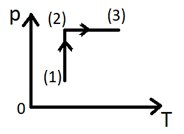
\includegraphics[scale=0.8]{../figs/VN10-2021-PH-TP032-13}
	\end{center}
	
}
\loigiai{
	Từ (1) sang (2) là quá trình đẳng nhiệt, áp suất tăng;
	
	Từ (2) sang (3) là quá trình đẳng áp, nhiệt độ tăng.
	
	Biểu diễn lại các quá trình trong hệ tọa độ $(V,T)$:
	\begin{center}
	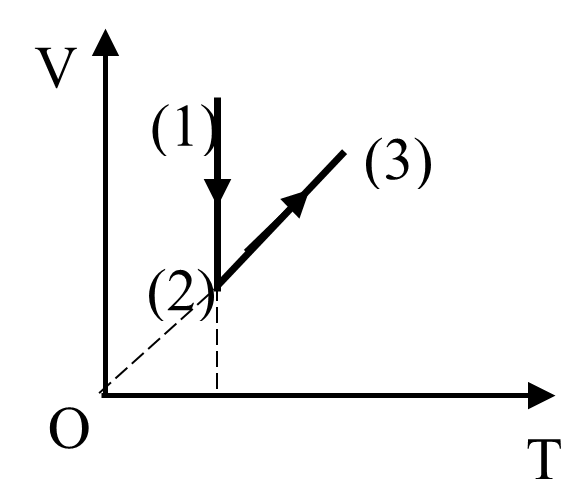
\includegraphics[scale=0.9]{../figs/VN10-2021-PH-TP032-14}
	\end{center}	
	
}



\item \mkstar{2} [14]

\cauhoi{
	Một khối khí lí tưởng biến đổi trạng thái qua hai quá trình liên tiếp được biểu diễn bằng đồ thị sau. Gọi tên các đẳng quá trình. Dựa vào các định luật hãy so sánh nhiệt độ ở trạng thái 1 với nhiệt độ ở trạng thái 3.
	\begin{center}
		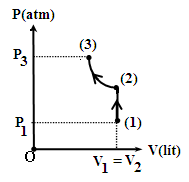
\includegraphics{../figs/VN10-2021-PH-TP032-16}
	\end{center}
	
}
\loigiai{
	
	Từ (1) sang (2): quá trình đẳng tích;
	
	Từ (2) sang (3): quá trình đẳng nhiệt.
	
	Từ (1) sang (2) áp suất tăng nên nhiệt độ tăng (áp suất tỉ lệ thuận với nhiệt độ). Vậy $T_2 > T_1$ suy ra $T_3>T_1$ (vì đẳng nhiệt $T_3=T_2$).
}
	\item \mkstar{2} [16]

\cauhoi{
	Một lượng khí đựng trong một xi lanh có pit-tông chuyển động được. Trạng thái của lượng khí lúc đầu là $\SI{2}{atm}$, $\SI{15}{l}$, $\SI{27}{\celsius}$. Khi pit-tông nén khí, áp suất của khí tăng lên tới $\SI{3.5}{atm}$, thể tích giảm còn $\SI{12}{l}$. Giả sử trong quá trình nén khí ở trên mà nhiệt độ khí không đổi, hãy vẽ đường đẳng nhiệt trong hệ trục $p\text{O}V$.
	
}
\loigiai{
	Vẽ đường đẳng nhiệt trong hệ trục $p\text{O}V$:
	\begin{center}
		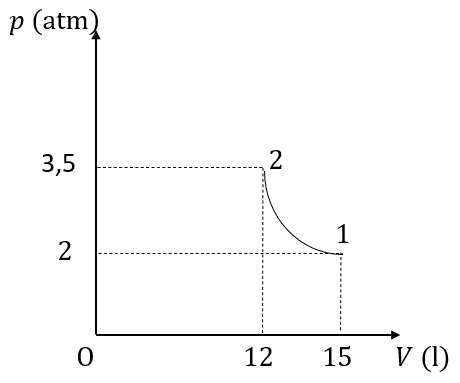
\includegraphics[scale=0.7]{../figs/VN10-2021-PH-TP032-18}
	\end{center}
}
\item \mkstar{2} [32]

\cauhoi{
	Một lượng khí lí tưởng biến đổi trạng thái như hình dưới.
	\begin{enumerate}[label=\alph*)]
		\item Gọi tên các quá trình biến đổi trạng thái của lượng khí trên.
		\item Tính thể tích ở trạng thái (1), biết thể tích ở trạng thái (2) là 10 lít.
	\end{enumerate}
	
	\begin{center}
		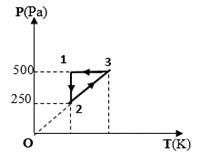
\includegraphics{../figs/VN10-2021-PH-TP032-22}
	\end{center}
}
\loigiai{
	
	\begin{enumerate}[label=\alph*)]
		\item Gọi tên các quá trình biến đổi trạng thái của lượng khí trên.
		
		Từ (1) sang (2): quá trình đẳng nhiệt;
		
		Từ (2) sang (3): quá trình đẳng tích;
		
		Từ (3) sang (1): quá trình đẳng áp.
		
		\item Tính thể tích ở trạng thái (1), biết thể tích ở trạng thái (2) là 10 lít.
		
		Đẳng nhiệt (1): $p_1=\SI{500}{Pa}$, $V_1=?$ sang (2): $p_2=\SI{250}{K}$, $V_2=\SI{10}{l}$
		
		Vì quá trình là đẳng nhiệt nên ta có phương trình:
		
		$$p_1V_1 = p_2V_2 \Rightarrow V_1 =\dfrac{p_2V_2}{p_1} = \SI{5}{l}.$$
	\end{enumerate}
}
		\item \mkstar{3} [1]
	
	\cauhoi{
		Một khối khí lí tưởng ở trạng thái ban đầu có áp suất $p_1=\SI{6}{atm}$, thể tích $V_1=\SI{2}{l}$ và nhiệt độ $t_1=\SI{27}{\celsius}$ biến đổi lần lượt qua các quá trình:
		\begin{itemize}
			\item Đẳng áp sang trạng thái 2 có nhiệt độ $t_2=\SI{627}{\celsius}$;
			\item Đẳng tích sang trạng thái 3 có áp suất $p_3=\SI{2}{atm}$;
			\item Đẳng nhiệt sang trạng thái 4 có thể tích $V_4=\SI{3}{l}$.
		\end{itemize}
		Vẽ đường biểu diễn các biến đổi trên trong hệ tọa độ $(\text{O}pV)$.
	}
	\loigiai{
		
		\begin{itemize}
			\item Đẳng áp (1): $p_1=\SI{6}{atm}$, $V_1=\SI{2}{l}$, $T_1=\SI{300}{K}$ sang (2): $p_2=p_1=\SI{6}{atm}$, $V_2=?$, $T_2=\SI{900}{K}$.
			
			Áp dụng phương trình trạng thái:
			
			$$\dfrac{p_1V_1}{T_1} = \dfrac{p_2V_2}{T_2} \Rightarrow V_2 =\dfrac{p_1V_1T_2}{p_2T_1} = \dfrac{V_1T_2}{T_1} = \SI{6}{l}.$$
			
			
			\item Đẳng tích (2): $p_2=\SI{6}{atm}$, $V_2=\SI{6}{l}$, $T_2=\SI{900}{K}$ sang (3): $p_3=\SI{2}{atm}$, $V_3=V_2=\SI{6}{l}$, $T_3=?$.
			
			Áp dụng phương trình trạng thái:
			
			$$\dfrac{p_2V_2}{T_2} = \dfrac{p_3V_3}{T_3} \Rightarrow T_3 =\dfrac{p_3V_3T_2}{p_2V_2}=\dfrac{p_3T_2}{p_2} =  \SI{300}{K}.$$
			
			
			\item Đẳng nhiệt (3): $p_3=\SI{2}{atm}$, $V_3=\SI{6}{l}$, $T_3=\SI{300}{K}$ sang (4): $p_4=?$, $V_4=\SI{3}{l}$, $T_4=T_3=\SI{300}{K}$.
			
			Áp dụng phương trình trạng thái:
			
			$$\dfrac{p_3V_3}{T_3} = \dfrac{p_4V_4}{T_4} \Rightarrow p_4 =\dfrac{p_3V_3T_4}{V_4T_3} = \dfrac{p_3V_3}{V_4} = \SI{4}{atm}.$$
			
			
		\end{itemize}
		Vẽ đường biểu diễn các biến đổi trên trong hệ tọa độ $(\text{O}pV)$:
		\begin{center}
			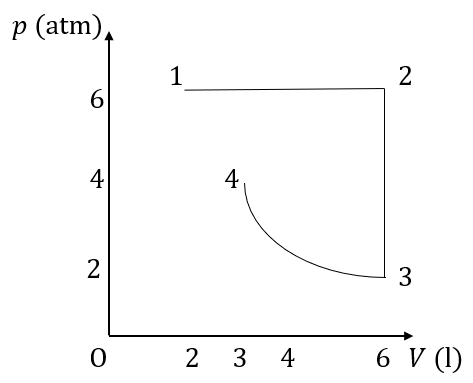
\includegraphics[scale=0.7]{../figs/VN10-2021-PH-TP032-7}
		\end{center}
	}
	\item \mkstar{3} [14]
	
	\cauhoi{
		Khi cho một lượng khí xác định được nén đẳng nhiệt từ thể tích $V_1=V_0$ sang thể tích $V_2=\dfrac{1}{3}V_0$ thì nhân thấy áp suất của lượng khí tăng thêm một lượng $\SI{2}{atm}$. Sau đó tiếp tục đun nóng đẳng tích đến khi nhiệt độ của khối khí tăng thêm $\SI{100}{\celsius}$ thì áp suất khối khí lúc này là $\SI{8}{atm}$. Vẽ đồ thị biểu diễn quá trình biến đổi các trạng thái trên trong hệ tọa độ $(\text{O}p,\text{O}T)$ với $\text{O}T$ là trục hoành.
	}
	\loigiai{
		
		Đẳng nhiệt (1): $p_1$, $V_1=V_0$, $T_1=?$ sang (2): $p_2=p_1 + \SI{2}{atm}$, $V_2=\dfrac{V_0}{3}$, $T_2=T_1$.
		
		Áp dụng phương trình trạng thái:
		
		$$\dfrac{p_1V_1}{T_1} = \dfrac{p_2V_2}{T_2} \Rightarrow p_1V_1 = p_2V_2 \Rightarrow p_1 V_0 = (p_1+2) \dfrac{1}{3}V_0 \Rightarrow p_1=\SI{1}{atm}.$$
		
		Đẳng tích (2): $p_2=p_1+\SI{2}{atm}=\SI{3}{atm}$, $V_2=\dfrac{1}{3}V_0$, $T_2=T_1$ sang (3): $p_3=\SI{8}{atm}$, $V_3=V_2=\dfrac{1}{3}V_0$, $T_3=T_2+\SI{100}{\celsius} = T_1 + \SI{100}{K}$.
		
		Áp dụng phương trình trạng thái:
		
		$$\dfrac{p_2V_2}{T_2} = \dfrac{p_3V_3}{T_3} \Rightarrow \dfrac{3}{T_1} = \dfrac{8}{T_1+100} \Rightarrow T_1 = \SI{60}{K}.$$
		
		Vẽ đồ thị biểu diễn quá trình biến đổi các trạng thái trên trong hệ tọa độ $(\text{O}p,\text{O}T)$ với $\text{O}T$ là trục hoành:
		\begin{center}
			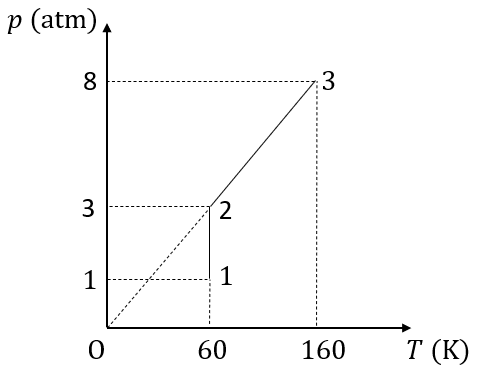
\includegraphics[scale=0.7]{../figs/VN10-2021-PH-TP032-17}
		\end{center}
	}

	\item \mkstar{3} [21]
	
	\cauhoi{
		Một khối khí lí tưởng có áp suất ban đầu $p_1$, thể tích 3 lít ở nhiệt độ $\SI{27}{\celsius}$ được biến đổi trạng thái qua hai quá trình liên tiếp nhau:
		\begin{itemize}
			\item Quá trình 1: làm lạnh đẳng tích để áp suất bằng $3/4$ áp suất ban đầu;
			\item Quá trình 2: nén đẳng nhiệt đến áp suất bằng $1/2$ áp suất ban đầu.
		\end{itemize}
	Biểu diễn các quá trình biến đổi trong hệ tọa độ $(p,V)$.
		
	}
	\loigiai{
		\begin{enumerate}[label=\alph*)]
			\item Tính nhiệt độ khí ở trạng thái (2) theo độ C.
			Đẳng tích (1): $p_1$, $V_1=\SI{3}{l}$, $T_1=\SI{300}{K}$ sang (2): $p_2=\dfrac{3}{4}p_1$, $V_2=V_1=\SI{3}{l}$, $T_2=?$.
			
			Áp dụng phương trình trạng thái:
			
			$$\dfrac{p_1V_1}{T_1} = \dfrac{p_2V_2}{T_2} \Rightarrow T_2=\dfrac{p_2V_2T_1}{p_1V_1} = \dfrac{p_2T_1}{p_1}=\SI{225}{K}.$$
			
			
			\item Tính thể tích khí ở trạng thái (3).
			Đẳng nhiệt (2): $p_2=\dfrac{3}{4}p_1$, $V_2=\SI{3}{l}$, $T_2=\SI{225}{K}$ sang (3): $p_3=\dfrac{1}{2}p_1$, $V_3=?$, $T_3=T_2$.
			
			Áp dụng phương trình trạng thái:
			
			$$\dfrac{p_2V_2}{T_2} = \dfrac{p_3V_3}{T_3} \Rightarrow V_3 = \dfrac{p_2V_2T_3}{p_3T_2} = \dfrac{p_2V_2}{p_3} = \SI{4.5}{l}.$$
		\end{enumerate}
	
	Biểu diễn các quá trình biến đổi trong hệ tọa độ $(p,V)$.
	\begin{center}
		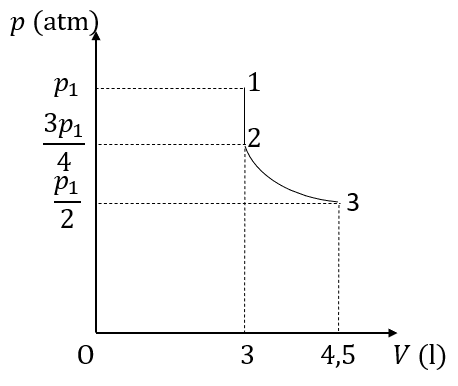
\includegraphics[scale=0.7]{../figs/VN10-2021-PH-TP032-19}
	\end{center}
	
	}

\item \mkstar{3} [23]

\cauhoi{
	Một lượng khí lí tưởng có áp suất $p_1=\SI{1}{atm}$, nhiệt độ $t_1=\SI{27}{\celsius}$ và thể tích $V_1=\SI{1}{l}$ biến đổi lần lượt qua hai quá trình sau:
	\begin{itemize}
		\item Biến đổi đẳng nhiệt tới thể tích $V_2=\SI{2}{l}$, áp suất $p_2$;
		\item Biến đổi đẳng tích tới áp suất $p_3=2p_2$, nhiệt độ $t_3$.
	\end{itemize}
	Vẽ đồ thị biểu diễn hai quá trình biến đổi trạng thái trên của khối khí trong hệ trục $(p,V)$.
}
\loigiai{
	Đẳng nhiệt (1): $p_1=\SI{1}{atm}$, $V_1=\SI{1}{l}$, $T_1=\SI{300}{K}$ sang (2): $p_2=?$, $V_2=\SI{2}{l}$, $T_2=T_1 = \SI{300}{K}$.
	
	Áp dụng phương trình trạng thái:
	
	$$\dfrac{p_1V_1}{T_1} = \dfrac{p_2V_2}{T_2} \Rightarrow p_2=\dfrac{p_1V_1T_2}{V_2T_1} = \dfrac{p_1V_1}{V_2}=\SI{0.5}{atm}.$$
	
	Đẳng tích (2): $p_2=\SI{0.5}{atm}$, $V_2=\SI{2}{l}$, $T_2=\SI{300}{K}$ sang (3): $p_3=2p_2=\SI{1}{atm}$, $V_3=V_2=\SI{2}{l}$, $T_3=?$.
	
	Áp dụng phương trình trạng thái:
	
	$$\dfrac{p_2V_2}{T_2} = \dfrac{p_3V_3}{T_3} \Rightarrow T_3=\dfrac{p_3V_3T_2}{p_2V_2} = \dfrac{p_3T_2}{p_2}=\SI{600}{K}.$$
	
	Vẽ đồ thị biểu diễn hai quá trình biến đổi trạng thái trên của khối khí trong hệ trục $(p,V)$:
	
	\begin{center}
		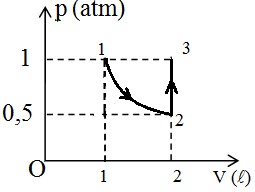
\includegraphics[scale=0.8]{../figs/VN10-2021-PH-TP032-20}
	\end{center}
}

\item \mkstar{3} [12]

\cauhoi{
	Một khối khí lí tưởng có nhiệt độ $\SI{27}{\celsius}$ ở trạng thái (1). Khí được biến đổi qua hai quá trình:
	\begin{itemize}
		\item Từ trạng thái (1), khí được biến đổi đẳng tích sang trạng thái (2) có áp suất $\SI{1.5}{atm}$ và nhiệt độ là $\SI{177}{\celsius}$, thể tích 10 lít.
		\item Từ trạng thái (2), khí được biến đổi đẳng áp sang trạng thái (3) có nhiệt độ $\SI{627}{\celsius}$.
	\end{itemize}
	Vẽ đồ thị biểu diễn quá trình biến đổi trạng thái trên trong hệ tọa độ $\text{O}p, \text{O}T$ với $\text{O}T$ là trục hoành, $\text{O}p$ là trục tung.
}
\loigiai{
	Đẳng tích (1): $p_1=?$, $V_1=\SI{10}{l}$, $T_1=\SI{300}{K}$ sang (2): $p_2=\SI{1.5}{atm}$, $V_2=V_1=\SI{10}{l}$, $T_2=T_1=\SI{450}{K}$.
	
	Áp dụng phương trình trạng thái:
	
	$$\dfrac{p_1V_1}{T_1} = \dfrac{p_2V_2}{T_2} \Rightarrow p_1 =\dfrac{p_2V_2T_1}{V_1T_2}=\dfrac{p_2T_1}{T_2} = \SI{1}{atm}.$$
	
	Đẳng áp (2): $p_2=\SI{1.5}{atm}$, $V_2=\SI{10}{l}$, $T_2=\SI{450}{K}$ sang (3): $p_3=p_2=\SI{1.5}{atm}$, $V_3=?$, $T_3=\SI{900}{K}$.
	
	Áp dụng phương trình trạng thái:
	
	$$\dfrac{p_2V_2}{T_2} = \dfrac{p_3V_3}{T_3} \Rightarrow V_3 =\dfrac{p_2V_2T_3}{T_2p_3}=\dfrac{V_2T_3}{T_2} = \SI{20}{l}.$$
	
	Vẽ đồ thị biểu diễn quá trình biến đổi trạng thái trên trong hệ tọa độ $\text{O}p, \text{O}T$ với $\text{O}T$ là trục hoành, $\text{O}p$ là trục tung.
	
	\begin{center}
		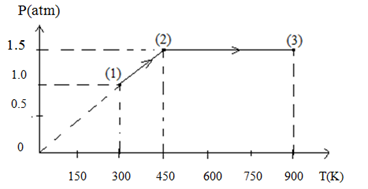
\includegraphics{../figs/VN10-2021-PH-TP032-21}
	\end{center}
	
}
\item \mkstar{3} [11]

\cauhoi{
	Một lượng khí lí tưởng ở nhiệt độ $\SI{27}{\celsius}$, áp suất $\SI{e5}{Pa}$, thể tích 4 lít được biến đổi trạng thái qua 2 giai đoạn: nén đẳng nhiệt đến áp suất là $\SI{2e5}{Pa}$, sau đó cho dãn nở đẳng áp đến thể tích $\SI{6}{l}$. Vẽ đồ thị mô tả quá trình biến đổi của khối khí trên trong hệ tọa độ $(p,T)$.
}
\loigiai{
	
	Đẳng nhiệt (1): $p_1=\SI{e5}{Pa}$, $V_1=\SI{4}{l}$, $T_1=\SI{300}{K}$ sang (2): $p_2=\SI{2e5}{Pa}$, $V_2=?$, $T_2=T_1=\SI{300}{K}$.
	
	Áp dụng phương trình trạng thái:
	
	$$\dfrac{p_1V_1}{T_1} = \dfrac{p_2V_2}{T_2} \Rightarrow V_2 =\dfrac{p_1V_1T_2}{p_2T_1}=\dfrac{p_1V_1}{p_2} = \SI{2}{l}.$$
	
	Đẳng áp (2): $p_2=\SI{2e5}{Pa}$ sang (3): $p_3=p_2=\SI{2e5}{Pa}$.
	
	Vẽ đồ thị mô tả quá trình biến đổi của khối khí trên trong hệ tọa độ $(p,T)$:
	\begin{center}
		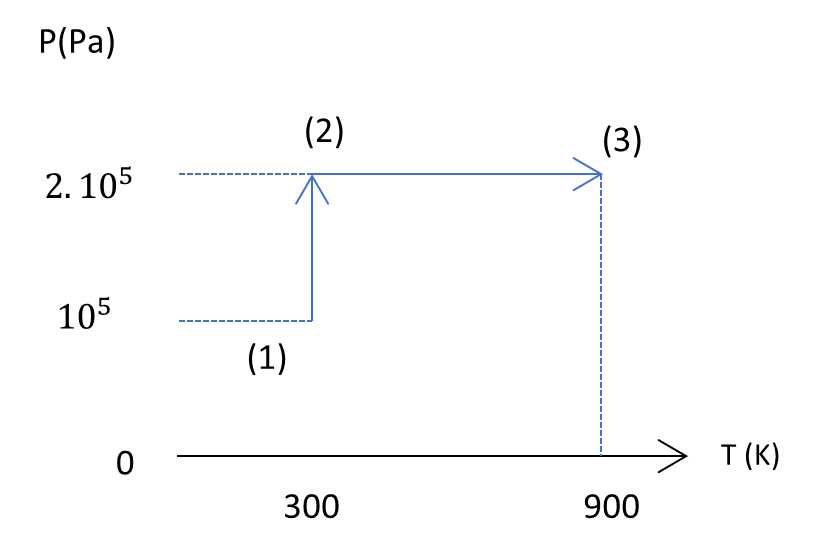
\includegraphics[scale=1.3]{../figs/VN10-2021-PH-TP032-23}
	\end{center}
}
\end{enumerate}	
\whiteBGstarEnd